\section{Scope, provenance, and evidence status}
This supplement documents the source snapshot used to assemble the manuscript.
It does not convert a protocol, a running job, or a workstation report into a completed endpoint.
The preparation script reads public aggregate JSONs, generates tables, copies selected population-summary PDFs, and records input hashes and producing commits in \src{evidence_manifest.json}.
No participant image or per-person result row is read during manuscript assembly.
Figure provenance describes the origin of the saved output; copying it does not independently reproduce the underlying experiment.

The labels \statusfinal\ and \statuspre\ apply to individual results and frames.
A frame can have an approved visual decision while an additional mask change remains unresolved.
An older run can contain valid measurements for its own question while being unsuitable as a replacement for the amended protocol.
The source-level status must therefore accompany every comparison, not just the dataset name.

\subsection{Coverage of the existing research materials}
\begin{table}[htbp]
\centering
\caption{Available cohorts and evidence status.
Units are target people for brain and faces, and target eyes for iris and P8/P9 fundus.
Independent clusters are families or people; the repeat column is endpoint-specific.
Sources: the saved brain, face, iris and frozen fundus metric/map aggregate files recorded in the evidence manifest.}
\label{tab:s-coverage}
\small
\begin{tabular}{@{}lrrll@{}}
\toprule
Dataset & Target units & Clusters & With repeat & Status \\
\midrule
QTIM & 221 & 168 & 23 & Affine, gate pending\statuspre \\
CelebA & 921 & 921 & Endpoint-specific & v6f frame approved\statusfinal \\
IMDb-WIKI & 678 & 453 & Endpoint-specific & v6f frame approved\statusfinal \\
UTIRIS NIR & 156 & 78 & 156 & P2 mask QC note\statuspre \\
UTIRIS VIS & 158 & 79 & 157 & P2 mask QC note\statuspre \\
UPOL & 128 & 64 & 128 & P2 mask QC note\statuspre \\
GRAPE P8 & 239 & 134 & 171 & Frame-only\statuspre \\
PAPILA P9 & 488 & 244 & Unavailable & Frame-only\statuspre \\
\bottomrule

\end{tabular}
\end{table}

The material inventory covers the tracked results, protocols, reports, figures and related ISBI source, with each artifact assigned a manuscript role.
Historical unregistered image-space and ocular pilots supply context for acquisition confounding, not substitutes for the current donor panels.
Fixed real-case demonstrations establish a preparation history rather than a population validation.
The synthetic population-null, label and pupil blocks are mechanism controls and remain separate from measured anatomy.
The earlier figure variants and failed preprocessing versions are retained as history rather than selected opportunistically for a favorable metric ordering.

The frozen bilateral-branch snapshot adds the P8/P9 fundus frame-only aggregate and its completed v1 metric registry.
Those files are preserved byte-for-byte in the paper inputs.
They are distinct from the still newer metric extension reported as running at handoff.
The inventory, source hashes and version distinctions are recorded in \src{MATERIALS_COVERAGE.md} and the evidence manifest.

\section{Population-audit questions and coverage}
Inpainting supplies controlled references for a proposed audit of conditional generation across target populations.
The twelve questions below separate the measured metric/reference evidence from the missing model-output validation.
No completion percentage, fairness result or universal metric follows from counting the rows.
BraTS~\cite{brats2023} is one application; cross-anatomy donor experiments do not themselves measure generator behavior across demographic groups.

{\small
\begin{longtable}{@{}p{.07\textwidth}p{.29\textwidth}p{.57\textwidth}@{}}
\caption{Population-audit questions, current evidence and missing validation.
Authored assessment from \src{population_audit.json}; source hashes are recorded in \src{population_audit_manifest.json}.}\\
\toprule
ID & Question and coverage & Evidence boundary and missing work \\
\midrule
\endfirsthead
\toprule
ID & Question and coverage & Evidence boundary and missing work \\
\midrule
\endhead
P01 & What is conditioned on, and which identity unit should be preserved?\par\emph{Task/reference definition developed} & Donor experiments distinguish person, eye, side and acquisition. Inpainting fixes visible context and permits observed-reference tests where a real region is hidden.\par\textbf{Missing:} A model-specific conditioning contract and an explicit treatment of unidentifiable detail. Human anatomical relationships need domain-specific replacements outside the current data. \\
P02 & Which target strata, donor cohorts and acquisition domains are being compared?\par\emph{Donor matching available; generator strata not measured} & Age/recorded-sex-matched means and family exclusion define reference cohorts. Accessible face tier-1 outputs do not establish a population-stratified audit of generated completions.\par\textbf{Missing:} Prespecified target groups, metadata availability, independent-unit counts and matched task-difficulty strata. A modality or dataset contrast is not a demographic disparity. \\
P03 & Is the distance implementation and support contract explicit?\par\emph{Substantial saved implementation-probe coverage} & Validity-mask tests and saved official inpainting-evaluator probes examine tensor layout, clipping, normalization and within-case ordering.\par\textbf{Missing:} Deployment parity and task-specific mask-boundary/three-dimensional conventions. A metric name alone does not specify an evaluator. \\
P04 & Does the score notice attenuation toward a global or matched population mean?\par\emph{Mechanism evidence; MRI provisional} & Known-target synthetic shrinkage and saved donor profiles separate low reference error from retained residual amplitude and target direction.\par\textbf{Missing:} Actual generated completions, information recoverable from their context and a distinction between legitimate mean prediction and harmful loss of relevant variation. \\
P05 & Can omitted detail be distinguished from plausible but incorrect detail?\par\emph{Controlled proxy evidence} & Norm-matched incorrect residuals, means and noise stress-test amplitude and alignment separately. Whole-image ArcFace evaluates face donor identity, not an inpainted composite.\par\textbf{Missing:} Paired model/control comparisons at the same spatial scope, independent anatomical error assessments and a defined cost of omission versus incorrect structure. \\
P06 & Is acquisition variation separated from identity or anatomy?\par\emph{Partial; MRI gate unresolved} & Repeat captures, paired contrast sensitivity and synthetic pupil changes supply nuisance controls. HACA3 contrast reduction does not demonstrate preservation of individual anatomy.\par\textbf{Missing:} Accepted correspondence/QC where needed and task-specific checks that nuisance invariance retains meaningful anatomy. \\
P07 & Are anatomical structure, downstream utility and spatial support tested?\par\emph{Synthetic/partial spatial evidence} & Threshold-segmentation and topology toys, Gaussian maps and historical size/shell sweeps provide mechanism and spatial diagnostics.\par\textbf{Missing:} Independent real-image structure/usefulness criteria, irregular masks and completed object-relative scale studies. Downstream agreement alone is not identity validation. \\
P08 & How does a generator compare with the ladder within each target stratum?\par\emph{Proposed readout; no subgroup generator experiment} & Existing controls provide candidate reference levels for paired comparisons. No valid shared-target, shared-mask model-output group profiles are present in the accessible snapshot.\par\textbf{Missing:} Frozen model outputs, matched eligible targets/support, sampling budgets and paired output-minus-control profiles for each metric, rung and target group. \\
P09 & Do apparent group differences survive a common reference and comparable task difficulty?\par\emph{Proposed comparison; not measured} & Global and metadata-matched donor means exist as distinct comparators. They motivate retaining both raw distances and common-reference versus within-group coordinates.\par\textbf{Missing:} Comparable mask/location/acquisition conditions, uncertainty in reference pools and group differences, and sensitivity to group-specific reference variance. Descriptive gaps are not causal fairness findings. \\
P10 & Are between-target variation and within-context sampling variation separated?\par\emph{Conceptual controls only} & Averaging and attenuation motivate the distinction, but saved donor averages are not samples from a trained generator.\par\textbf{Missing:} Repeated outputs at a fixed seed/sample budget, conditional diversity and target-specific fidelity measurements. Reduced variance or mean preference alone does not establish mode collapse. \\
P11 & Do profiles support stable, independently meaningful evaluation decisions?\par\emph{Metric dependence partial; model/group decisions unvalidated} & Rung correlations, source intervals and toy rank probes exist. They are not confidence intervals for method rankings or group disparities.\par\textbf{Missing:} Independent quality criteria, target-cluster uncertainty with repeated masks/seeds, eligibility/missingness and worst-group summaries where estimable, and frozen aggregation choices. \\
P12 & Which parts transfer beyond inpainting to other generative settings?\par\emph{Proposed extension; human-anatomy evidence only} & Inpainting exposes context, withheld content and population controls in a paired task. These components can define an audit where a broader generator has an identity-bearing condition and meaningful reference unit.\par\textbf{Missing:} New domain-specific controls and validation. Unconditional generation has no intended target individual; paired identity fidelity cannot be applied without that condition and requires separate distribution/coverage criteria. \\
\bottomrule

\end{longtable}
}

The historical \src{results/real_cases.json} and \src{results/real_cases_parietal.json} explicitly withdraw all their c, correlation and label results because of an incorrect intensity-scaling peak.
They are excluded from the coverage supporting current conclusions, rather than retained as provisional evidence.
Protocols mentioning challenge models, fixed illustrations, and available model code do not establish a completed comparison of predictions.

\subsection{Target populations and reference cohorts}
The face protocol defines matched donor means using the recorded Male/Young attributes in CelebA and sex/age bands in IMDb-WIKI.
The brain protocol likewise defines sex/age-matched reference cohorts with family exclusion.
These are comparator definitions; the accessible aggregates do not establish a population-stratified experiment on generated completions.
The initial face protocol's strata-not-run statement describes that version's output specification, not every later or unreceived private run.
Iris sex/age matching is unavailable without the corresponding metadata.

Target strata, donor cohorts and acquisition domains must be specified separately.
For the proposed generator profile, average outputs within each target before the target-population average, fix support independently of generated content, retain common cross-model target/mask eligibility, and report failures.
Paired distances require an observed target and explicit fill/composite/whole-image scope; FID/FWD are set-level measures requiring a separate definition.
Common-reference and stratum-matched profiles should accompany raw distances and coverage, since group-specific reference variability can alter calibrated coordinates.
Neither low residual amplitude nor a group gap alone demonstrates mode collapse or causal discrimination.
Unconditional generation and unobserved counterfactual targets require criteria beyond paired target fidelity.

\subsection{Saved official-evaluator implementation probes}
The source probes use \texttt{inpainting} 0.0.12 and one constructed volume, with eleven fills spanning noise, blur, a constant mean, gain and overshoot.
The recorded input shape is $[1,40,48,36]$.
The first anatomical axis is interpreted as channels by the two-dimensional SSIM call; jointly permuting it in every input leaves the score unchanged.
This establishes an implementation convention rather than an empirical judgment that every two-dimensional SSIM is unsuitable.

\begin{table}[htbp]
\centering
\caption{Saved synthetic evaluator probes under two dependency versions.
SSIM lists the original score and joint first-axis permutation; PSNR lists the reported score and the expression using unclamped squared error, in dB.
The last column lists Kendall agreement with RMSE for plain PSNR and its epsilon variant across the eleven fills.
Sources: \src{results/brats_panel_checks_tm1.1.2.json} and \src{results/brats_panel_checks_tm1.9.0.json}.}
\small
\begin{tabular}{@{}lccc@{}}
\toprule
Torchmetrics & SSIM original / permuted & PSNR / unclamped & $\tau$: plain / epsilon \\
\midrule
1.1.2 & 0.956163 / 0.956163 & 12.317 / 9.091 & 0.891 / 1.000 \\
1.9.0 & 0.956163 / 0.956163 & 12.317 / 9.091 & 0.891 / 1.000 \\
\bottomrule

\end{tabular}
\end{table}

For a fixed case and the same error definition, PSNR is monotone in MSE.
The plain recorded implementation instead clips predictions to the reference's in-mask range; the probe therefore breaks exact rank identity.
This difference should not be interpreted as independent evidence of anatomical sensitivity.
Rung correlations, synthetic fill-order agreement and cluster bootstrap intervals do not establish stability of a leaderboard over reconstruction methods.
Scoring multiple stochastic predictions additionally requires a fixed output count, sampling budget and selection/aggregation rule; these have not been evaluated here.

\section{Distances, units, and aggregation}
\subsection{Mean-relative error and finite references}
The mean-relative unit divides the sum of eligible candidate errors by the sum of mean-fill errors on the same support.
An average of ratios can overweight nearly information-free targets and is not substituted for this quantity.
The additive equal-variance model gives the familiar reference errors $V$ for a population expectation and $2V$ for an independent donor.
A finite leave-person-out mean introduces estimation variance, and differing masks change which target distribution is summarized.
The stranger-to-mean ratio is therefore a diagnostic check, not a normalization identity forced to equal two.
Under the same additive, equal-variance assumptions, $1-Q/2$ estimates a shared residual correlation.
It is not an empirical estimate of heritability or a probability of preserved identity when those assumptions fail.

For other distances, the relevant baseline is empirical.
MSE and RMSE retain the same ordering within a fixed target despite differing raw aggregation and anchored coordinates.
PSNR has the corresponding monotonicity only with the recorded range and clamping rules held fixed.
For unit-normalized features, squared Euclidean distance is twice cosine distance, so their rank agreement is not independent evidence of validity.

\subsection{Intensity adaptations of structural scores}
The TM-like score adapts the continuous kernel of TM-score~\cite{tmscore2004} to each eligible intensity difference $\delta_v=f(v)-x(v)$:
\begin{equation}
S_{\rm TM}=\frac{1}{|E|}\sum_{v\in E}\frac{1}{1+(|\delta_v|/\sigma_{\rm rep})^2}.
\end{equation}
Here $\sigma_{\rm rep}$ is the pooled repeat-pair RMSE at the same position and side, excluding the target family and requiring at least five other pairs.
The GDT-like intensity score averages the proportions satisfying $|\delta_v|<m\sigma_{\rm rep}$ for $m\in\{0.5,1,2,4\}$.
The repeat-normalized RMSE divides RMSE by the same tolerance.
No valid repeat tolerance means an unavailable cell, not a score of zero.

The lDDT-like adaptation~\cite{lddt2013} compares local intensity differences, not inter-atomic distances.
For each eligible neighboring voxel pair $(u,v)$ within radius two in voxel coordinates, it measures
$|(f(u)-f(v))-(x(u)-x(v))|$.
The score averages the fractions below the four thresholds $m\sigma_{\rm rep}$.
Its original fixed-tolerance variant instead uses $\{0.25,0.5,1,2\}$ standardized intensity units.
These scores increase with similarity and are oriented before computing the reported distance coordinates.
A constant offset leaves the intensity-difference score unchanged; this invariance does not establish anatomical correctness.

\subsection{Residual magnitude and direction}
For target residual $a=x-\hat\mu$ and candidate residual $b=f-\hat\mu$, magnitude and target projection are
\begin{equation}
A=\frac{\|b\|}{\|a\|},\qquad
P=\frac{\langle b,a\rangle}{\|a\|^2}.
\end{equation}
An orthogonal residual can have $A=1$ and $P=0$.
On the known-target shrinkage path $b=\lambda a$, both coordinates equal $\lambda$, while residual cosine remains one for positive $\lambda$.
These algebraic identities explain the controls but are not independent validation.
A small target residual relative to acquisition variability makes the ratios unstable and needs an explicit resolution rule.

\section{Validity masks and Gaussian spatial reporting}
Missing observations retain their own masks through registration, normalization, donor averaging, context matching and local scoring.
The mean intensity outside an image is not zero just because the stored canvas contains zeros.
Selection-based donors are especially sensitive: a candidate must not win a context search because its padding accidentally matches the standardized target.
The saved fundus block-search outputs preceding this correction are omitted from the manuscript.

Local-error displays use normalized masked Gaussian averages.
Their standard deviation matches the variance of the recorded width through $w/\sqrt{12}$.
Binary box-support fractions can still define eligibility; this does not turn displayed errors into box averages.
Fine brain maps and the coarser look-alike grid have different sampling and interpolation, which must remain visible in provenance.
For fundus fixed-composition maps, all displayed positions retain the same set of contributing targets to reduce spatial composition artifacts.
This reduces one artifact class and does not establish anatomical validity.

\paragraph{Display of the main MRI panels.}
For the main illustration only, one common exterior display mask is derived from the six rendered MRI panels.
Only border-connected locations that are black, white or transparent in every panel are made transparent; enclosed dark anatomy is retained.
One tight crop and a light outer boundary are applied uniformly, preserving retained pixel colors.
This display mask is not an acquisition or measurement mask and does not change errors, eligibility or window definitions.
The numeric color limits remain $0$, $1$ and $2.4$; V retains its own row-specific display range.
Source, illustration, crop and pixel-preservation records are in \src{provenance_infographic_v2.json}.

\begin{figure*}[t]
\centering
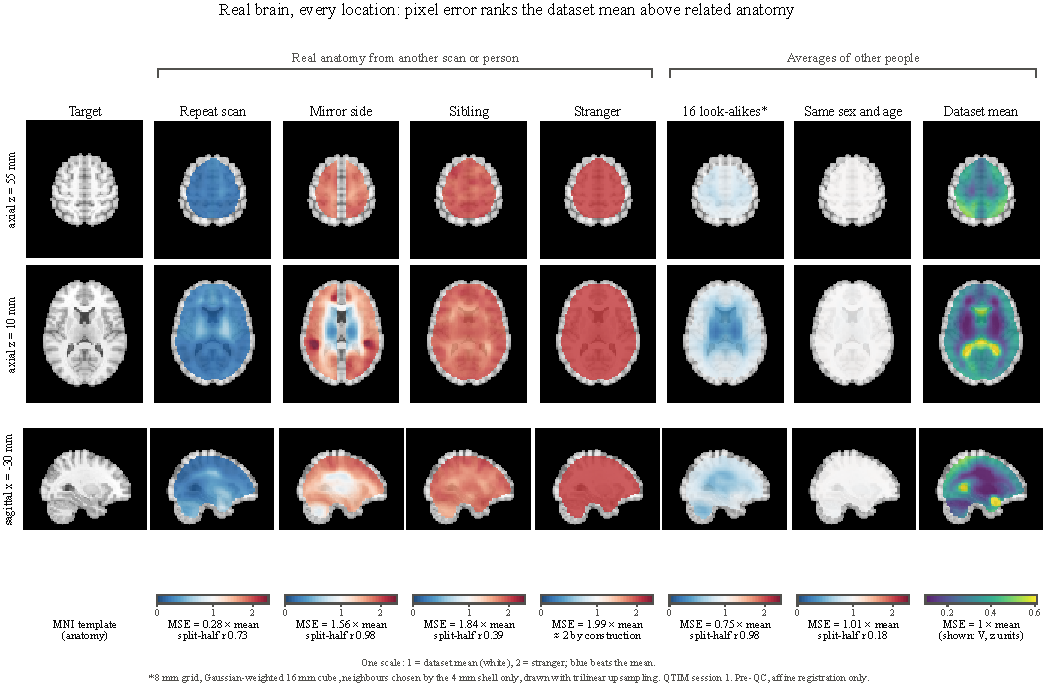
\includegraphics[width=\textwidth]{fig/brain_gaussian_maps.pdf}
\caption{\textbf{Saved provisional Gaussian brain maps.}
Population-template anatomy underlies aggregated donor-error maps.
The source remains pre-QC with affine registration.
Displayed local errors use the Gaussian amendments; the coarser look-alike grid is interpolated for display.
The source image title is a descriptive pixel-error statement, not a validated biological identity conclusion.
Source figure: \src{results/figures/fig_ladder_maps_common.pdf}; quantitative sources are the brain map and map-grid JSONs.}
\label{fig:s-brain}
\end{figure*}


\section{Directional tests and uncertainty}
The recorded tests have explicit reference candidates.
T1 compares repeat with dataset mean; T2 compares repeat with its attenuated version; T3a compares repeat with incorrect detail; T3b compares repeat with white noise.
The paired independent unit is a family for QTIM and a person for iris.
The fundus v1 panel uses a repeat reference for GRAPE and a fellow-eye reference for PAPILA; PAPILA has no T1 comparison.
The corresponding source protocol specifies its Holm family, and unavailable comparisons retain their status rather than becoming successful tests.

\begin{table*}[t]
\centering
\caption{\textbf{Recorded brain directional tests, provisional.}
Each cell reports the source decision and Holm-adjusted probability.
The test is one-sided in favor of the repeat.
Not establishing T2 is not an equivalence result.
Residual correlation versus the exact mean has no eligible T1 pair.
Source: \src{results/donor_ladder_brain_metrics.json}, random-region LR view.}
\small
\begin{tabular}{@{}lcccc@{}}
\toprule
Metric & T1 & T2 & T3a & T3b \\
\midrule
MSE & pass (6.6e-06)\statuspre & not established (1)\statuspre & pass (6.6e-06)\statuspre & pass (6.6e-06)\statuspre \\
SSIM & pass (6.6e-06)\statuspre & not established (1)\statuspre & pass (6.6e-06)\statuspre & pass (6.6e-06)\statuspre \\
Residual correlation & \notrun & not established (1)\statuspre & pass (6.6e-06)\statuspre & pass (6.6e-06)\statuspre \\
TM-like & pass (6.6e-06)\statuspre & not established (1)\statuspre & pass (6.6e-06)\statuspre & pass (6.6e-06)\statuspre \\
lDDT-like, repeat tolerance & pass (6.6e-06)\statuspre & not established (1)\statuspre & pass (6.6e-06)\statuspre & pass (6.6e-06)\statuspre \\
\bottomrule

\end{tabular}
\end{table*}

Source intervals resample independent clusters and, where specified, positions.
The cluster-only interval retained in the source answers a different uncertainty question from the two-way interval.
Neither interval repairs registration bias or an incorrect identity definition.
No new confidence interval or hypothesis test is recomputed from the published aggregate summaries.

\section{Available metric registry}
The fixed registry distinguishes computed, blocked and unavailable metrics before a ranking is interpreted.
The following table compares the completed fundus v1 registry with the accessible iris P2 registry.
A later unblocking amendment does not change these historical run statuses.
The main brain table uses its own tier-1 definitions and resampling scheme.

{\small
\begin{longtable}{@{}lll@{}}
\caption{Metric availability in the frozen sources.
Sources: \src{results/fundus_ladder_metrics.json} at the bilateral snapshot and \src{results/iris_ladder_metrics.json}.}\\
\toprule
Metric & Fundus v1 & Iris P2 \\
\midrule
\endfirsthead
\toprule
Metric & Fundus v1 & Iris P2 \\
\midrule
\endhead
mse & computed & computed \\
rmse & computed & computed \\
psnr & computed & computed \\
mae & computed & computed \\
ssim & computed & computed \\
ms\_ssim & computed & computed \\
lpips & blocked & blocked \\
acc\_dataset & computed & computed \\
acc\_matched & computed & blocked \\
amplitude\_dataset & computed & computed \\
amplitude\_matched & computed & blocked \\
lddt & computed & computed \\
intensity\_persistence & computed & computed \\
betti\_matching\_matched & blocked & blocked \\
betti\_matching\_unmatched & blocked & blocked \\
id\_angle & blocked & blocked \\
id\_norm & blocked & blocked \\
id\_pfe & blocked & blocked \\
id\_plda & blocked & blocked \\
latent\_pullback & blocked & blocked \\
latent\_fisher\_rao & blocked & blocked \\
latent\_lddmm & blocked & blocked \\
plausibility & blocked & blocked \\
fid & blocked & blocked \\
fwd & blocked & blocked \\
topology\_distance & blocked & blocked \\
\bottomrule

\end{longtable}
}

\clearpage
\section{CARE aggregation audit as related evidence}
The repository also contains a separate reproduction attempt on the released CARE scores~\cite{care2025}.
Its current iteration records the status of each published median/quartile comparison under the frozen aggregation rule.
This is a consistency audit of released scores, not generation of reconstructed CT or a rerun of the image-level segmenter.
An aggregation mismatch does not refute the anatomical benefit of the reconstruction method.
Coverage failures and non-finite values remain distinct from numeric disagreement.

\begin{table}[htbp]
\centering
\caption{Saved CARE iteration-2 comparison statuses, counted directly from the source rows.
Source: \src{results/care_iteration2.json}.
The status names refer to the recorded numerical comparison, not the validity of CARE's broader scientific claims.}
\begin{tabular}{@{}lr@{}}
\toprule
Recorded comparison status & Count \\
\midrule
Within the recorded rounding tolerance & 36 \\
Outside that tolerance & 63 \\
Blocked by coverage & 8 \\
No finite available comparison & 1 \\
\bottomrule

\end{tabular}
\end{table}

\section{Correlation and historical size sensitivity}
The saved correlation analysis groups distances by their rung-order dependence within target, position and side.
Strong agreement among monotone variants is not independent confirmation of identity sensitivity.
The saved size/shell sweep varies older window and context choices; it is not the completed object-relative sweep specified by the latest amendment.
Both figures remain provisional and retain the source protocol's interpretation.

\clearpage
\begin{figure}[p]
\centering
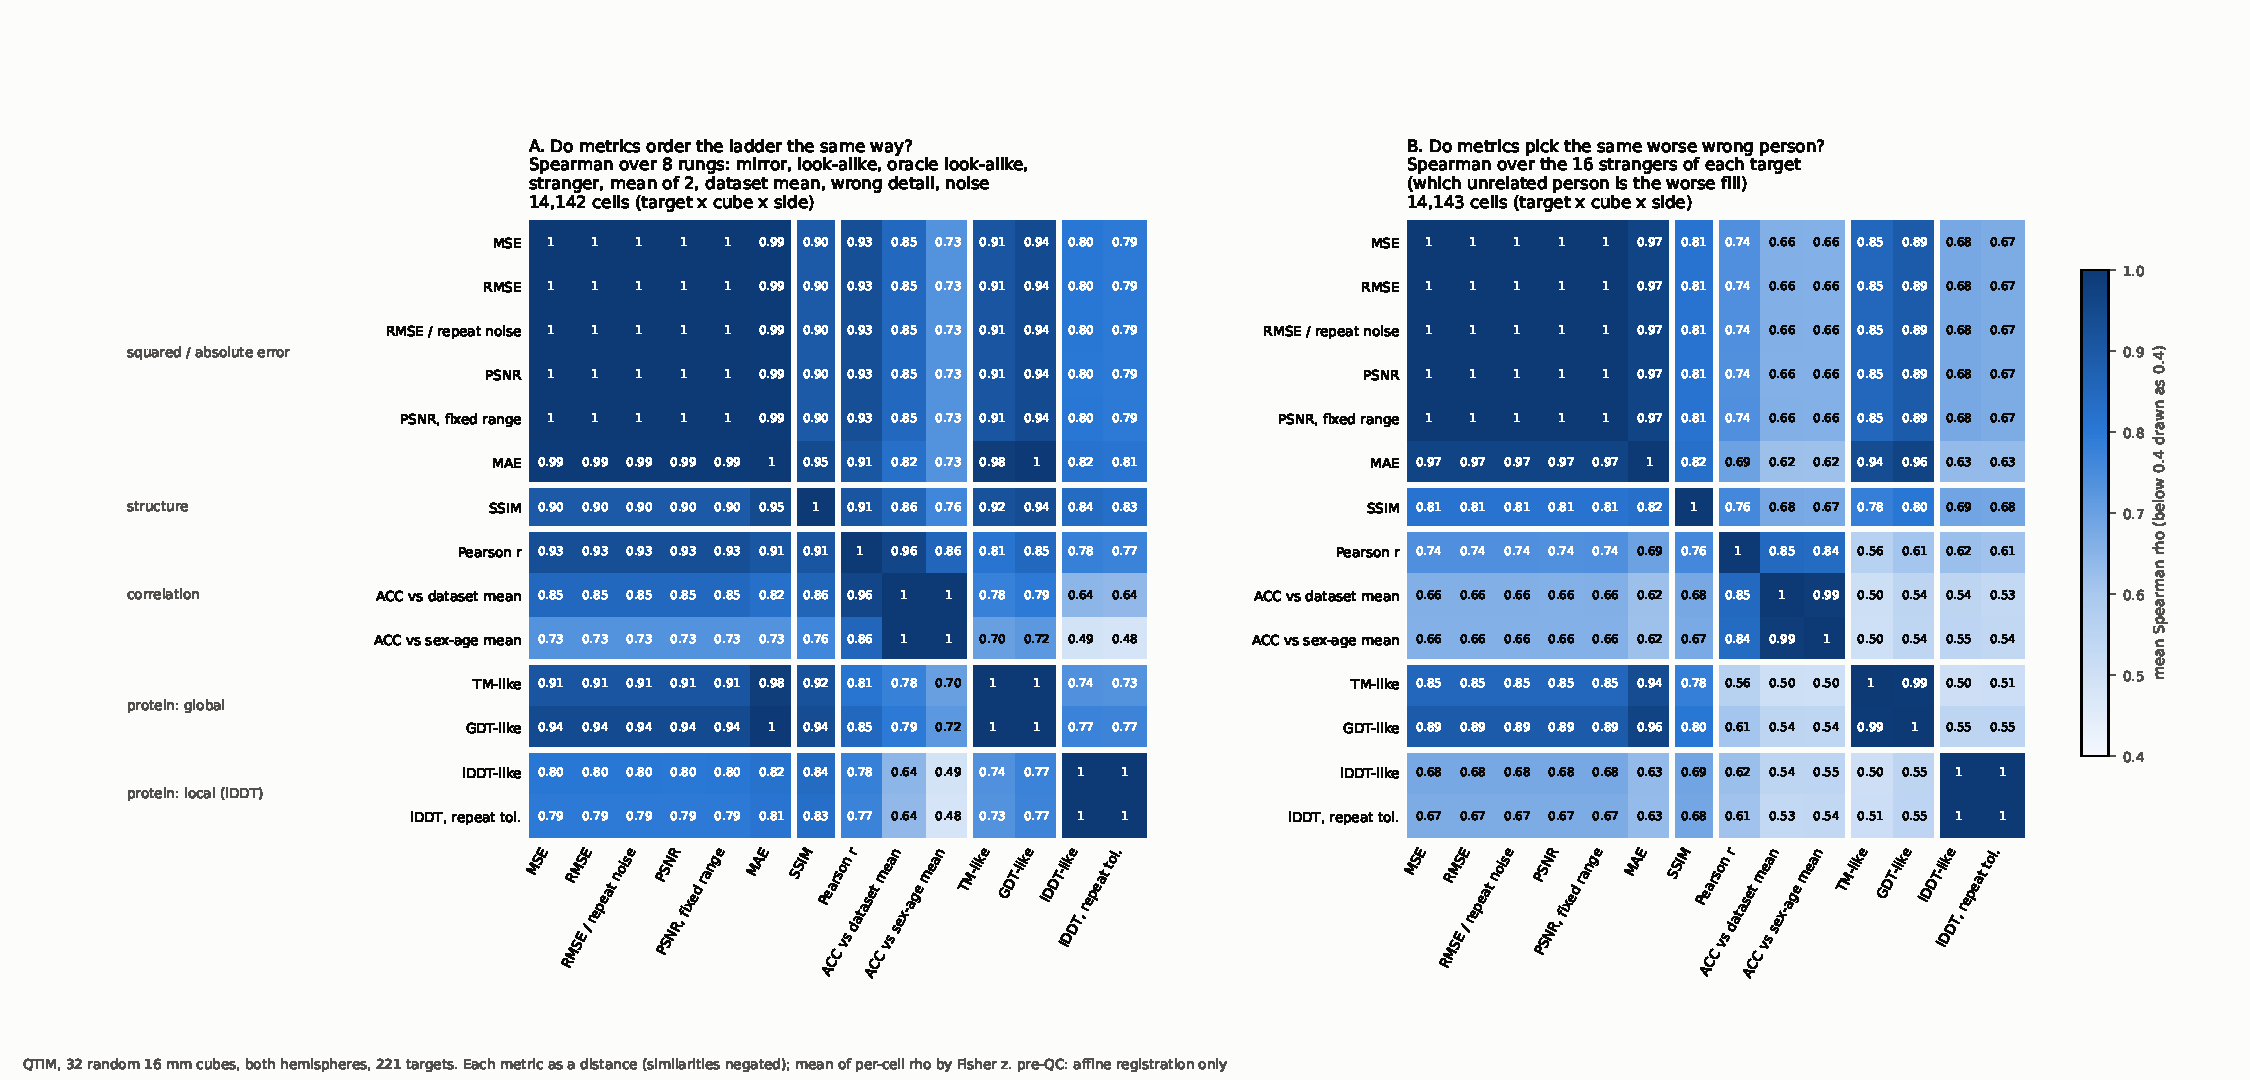
\includegraphics[width=.9\textwidth,height=.72\textheight,keepaspectratio]{fig/metric_correlations.pdf}
\caption{Saved provisional metric-dependence analysis.
Source: \src{results/figures/fig_metrics_correlation.pdf}, with \src{results/donor_ladder_metrics_correlation.json}.
This is descriptive dependence among measures, not a learned fusion or a ranking of validated identity metrics.}
\end{figure}

\clearpage
\begin{figure}[p]
\centering
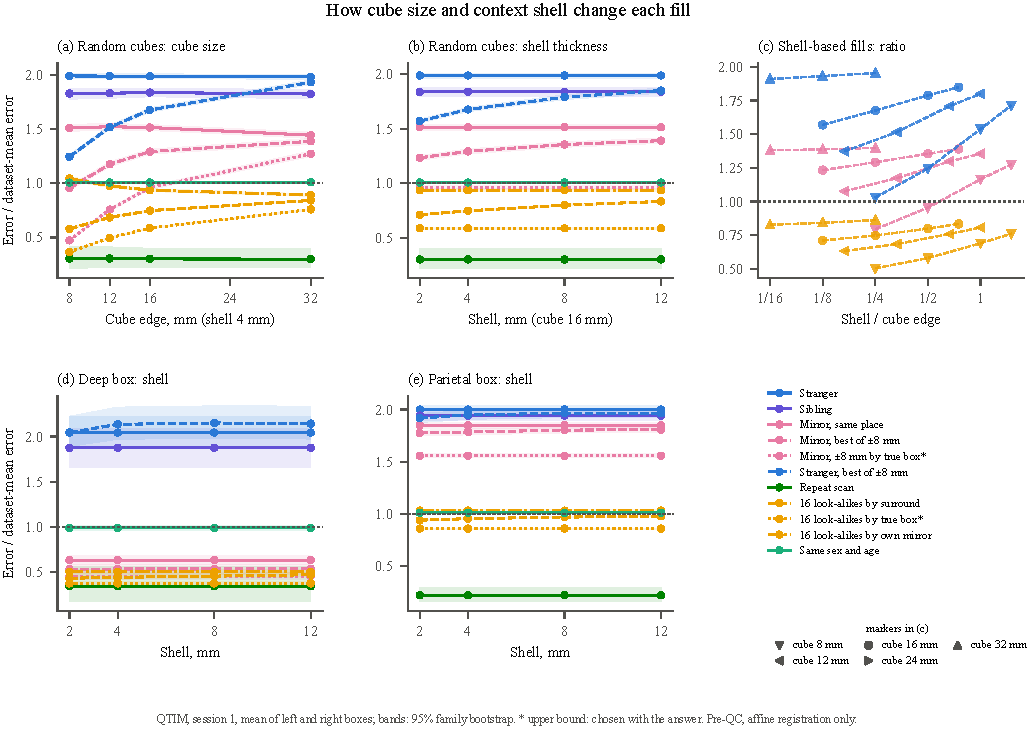
\includegraphics[width=.95\textwidth,height=.72\textheight,keepaspectratio]{fig/size_shell_sensitivity.pdf}
\caption{Saved provisional window/context sensitivity from the earlier sweep.
Source: \src{results/figures/fig_size_shell_dependence.pdf}, with \src{results/donor_ladder_brain_size.json}.
The figure does not establish completion of the latest object-relative metric-panel sweep.}
\end{figure}
\clearpage

\section{Full selected brain profiles}
Table~\ref{tab:s-brain-full} preserves endpoint-specific target and family counts for the selected rungs across all available tier-1 distances.
These are provisional random-region LR values and do not replace a post-registration panel.

{\small
\begin{longtable}{@{}llcrr@{}}
\caption{Selected saved brain $R_{\rm rep}$ profiles and 95\% intervals.
Source: \src{results/donor_ladder_brain_metrics.json}.}
\label{tab:s-brain-full}\\
\toprule
Metric & Rung & $R_{\rm rep}$ & Targets & Families \\
\midrule
\endfirsthead
\toprule
Metric & Rung & $R_{\rm rep}$ & Targets & Families \\
\midrule
\endhead
mse & dataset\_mean & \shortstack{0.413\statuspre\\{\scriptsize [0.367, 0.443]}} & 221 & 168 \\
mse & mirror & \shortstack{0.717\statuspre\\{\scriptsize [0.622, 0.792]}} & 221 & 168 \\
mse & repeat & \shortstack{0.000\statuspre\\{\scriptsize [0.000, 0.000]}} & 23 & 23 \\
mse & shrink\_repeat & \shortstack{-0.014\statuspre\\{\scriptsize [-0.028, -0.004]}} & 23 & 23 \\
mse & wrong\_detail & \shortstack{1.006\statuspre\\{\scriptsize [0.992, 1.020]}} & 221 & 168 \\
mse & noise & \shortstack{0.921\statuspre\\{\scriptsize [0.893, 0.944]}} & 221 & 168 \\
rmse & dataset\_mean & \shortstack{0.538\statuspre\\{\scriptsize [0.488, 0.573]}} & 221 & 168 \\
rmse & mirror & \shortstack{0.766\statuspre\\{\scriptsize [0.682, 0.830]}} & 221 & 168 \\
rmse & repeat & \shortstack{0.000\statuspre\\{\scriptsize [0.000, 0.000]}} & 23 & 23 \\
rmse & shrink\_repeat & \shortstack{-0.015\statuspre\\{\scriptsize [-0.031, -0.002]}} & 23 & 23 \\
rmse & wrong\_detail & \shortstack{1.001\statuspre\\{\scriptsize [0.993, 1.010]}} & 221 & 168 \\
rmse & noise & \shortstack{0.943\statuspre\\{\scriptsize [0.924, 0.958]}} & 221 & 168 \\
mae & dataset\_mean & \shortstack{0.554\statuspre\\{\scriptsize [0.495, 0.595]}} & 221 & 168 \\
mae & mirror & \shortstack{0.702\statuspre\\{\scriptsize [0.593, 0.784]}} & 221 & 168 \\
mae & repeat & \shortstack{0.000\statuspre\\{\scriptsize [0.000, 0.000]}} & 23 & 23 \\
mae & shrink\_repeat & \shortstack{-0.014\statuspre\\{\scriptsize [-0.033, 0.000]}} & 23 & 23 \\
mae & wrong\_detail & \shortstack{0.997\statuspre\\{\scriptsize [0.987, 1.007]}} & 221 & 168 \\
mae & noise & \shortstack{0.997\statuspre\\{\scriptsize [0.970, 1.031]}} & 221 & 168 \\
psnr & dataset\_mean & \shortstack{0.664\statuspre\\{\scriptsize [0.611, 0.702]}} & 221 & 168 \\
psnr & mirror & \shortstack{0.815\statuspre\\{\scriptsize [0.744, 0.870]}} & 221 & 168 \\
psnr & repeat & \shortstack{0.000\statuspre\\{\scriptsize [0.000, 0.000]}} & 23 & 23 \\
psnr & shrink\_repeat & \shortstack{-0.014\statuspre\\{\scriptsize [-0.036, 0.004]}} & 23 & 23 \\
psnr & wrong\_detail & \shortstack{1.000\statuspre\\{\scriptsize [0.994, 1.005]}} & 221 & 168 \\
psnr & noise & \shortstack{0.963\statuspre\\{\scriptsize [0.950, 0.973]}} & 221 & 168 \\
psnr\_fixed & dataset\_mean & \shortstack{0.666\statuspre\\{\scriptsize [0.613, 0.704]}} & 221 & 168 \\
psnr\_fixed & mirror & \shortstack{0.816\statuspre\\{\scriptsize [0.744, 0.872]}} & 221 & 168 \\
psnr\_fixed & repeat & \shortstack{0.000\statuspre\\{\scriptsize [0.000, 0.000]}} & 23 & 23 \\
psnr\_fixed & shrink\_repeat & \shortstack{-0.014\statuspre\\{\scriptsize [-0.035, 0.004]}} & 23 & 23 \\
psnr\_fixed & wrong\_detail & \shortstack{1.000\statuspre\\{\scriptsize [0.994, 1.005]}} & 221 & 168 \\
psnr\_fixed & noise & \shortstack{0.963\statuspre\\{\scriptsize [0.950, 0.974]}} & 221 & 168 \\
ssim & dataset\_mean & \shortstack{0.738\statuspre\\{\scriptsize [0.680, 0.784]}} & 221 & 168 \\
ssim & mirror & \shortstack{0.823\statuspre\\{\scriptsize [0.755, 0.873]}} & 221 & 168 \\
ssim & repeat & \shortstack{0.000\statuspre\\{\scriptsize [0.000, 0.000]}} & 23 & 23 \\
ssim & shrink\_repeat & \shortstack{0.001\statuspre\\{\scriptsize [-0.015, 0.016]}} & 23 & 23 \\
ssim & wrong\_detail & \shortstack{1.023\statuspre\\{\scriptsize [1.014, 1.036]}} & 221 & 168 \\
ssim & noise & \shortstack{1.132\statuspre\\{\scriptsize [1.088, 1.194]}} & 221 & 168 \\
pearson & dataset\_mean & \shortstack{0.581\statuspre\\{\scriptsize [0.547, 0.610]}} & 221 & 168 \\
pearson & mirror & \shortstack{0.817\statuspre\\{\scriptsize [0.757, 0.869]}} & 221 & 168 \\
pearson & repeat & \shortstack{0.000\statuspre\\{\scriptsize [0.000, 0.000]}} & 23 & 23 \\
pearson & shrink\_repeat & \shortstack{-0.005\statuspre\\{\scriptsize [-0.009, -0.003]}} & 23 & 23 \\
pearson & wrong\_detail & \shortstack{1.013\statuspre\\{\scriptsize [1.002, 1.026]}} & 221 & 168 \\
pearson & noise & \shortstack{0.989\statuspre\\{\scriptsize [0.985, 0.994]}} & 221 & 168 \\
acc\_dataset & dataset\_mean & \textit{undefined} & \textit{undefined} & \textit{undefined} \\
acc\_dataset & mirror & \shortstack{0.752\statuspre\\{\scriptsize [0.688, 0.808]}} & 221 & 168 \\
acc\_dataset & repeat & \shortstack{0.000\statuspre\\{\scriptsize [0.000, 0.000]}} & 23 & 23 \\
acc\_dataset & shrink\_repeat & \shortstack{-0.000\statuspre\\{\scriptsize [-0.000, 0.000]}} & 23 & 23 \\
acc\_dataset & wrong\_detail & \shortstack{1.003\statuspre\\{\scriptsize [0.996, 1.009]}} & 221 & 168 \\
acc\_dataset & noise & \shortstack{1.003\statuspre\\{\scriptsize [1.000, 1.006]}} & 221 & 168 \\
acc\_cohort & dataset\_mean & \shortstack{0.893\statuspre\\{\scriptsize [0.883, 0.903]}} & 221 & 168 \\
acc\_cohort & mirror & \shortstack{0.755\statuspre\\{\scriptsize [0.691, 0.811]}} & 221 & 168 \\
acc\_cohort & repeat & \shortstack{0.000\statuspre\\{\scriptsize [0.000, 0.000]}} & 23 & 23 \\
acc\_cohort & shrink\_repeat & \shortstack{-0.000\statuspre\\{\scriptsize [-0.000, 0.000]}} & 23 & 23 \\
acc\_cohort & wrong\_detail & \shortstack{1.003\statuspre\\{\scriptsize [0.995, 1.009]}} & 221 & 168 \\
acc\_cohort & noise & \shortstack{1.001\statuspre\\{\scriptsize [0.999, 1.004]}} & 221 & 168 \\
lddt & dataset\_mean & \shortstack{0.375\statuspre\\{\scriptsize [0.301, 0.434]}} & 221 & 168 \\
lddt & mirror & \shortstack{0.889\statuspre\\{\scriptsize [0.842, 0.925]}} & 221 & 168 \\
lddt & repeat & \shortstack{0.000\statuspre\\{\scriptsize [0.000, 0.000]}} & 23 & 23 \\
lddt & shrink\_repeat & \shortstack{-0.069\statuspre\\{\scriptsize [-0.088, -0.053]}} & 23 & 23 \\
lddt & wrong\_detail & \shortstack{1.056\statuspre\\{\scriptsize [1.034, 1.086]}} & 221 & 168 \\
lddt & noise & \shortstack{2.159\statuspre\\{\scriptsize [2.013, 2.347]}} & 221 & 168 \\
tm\_like & dataset\_mean & \shortstack{0.723\statuspre\\{\scriptsize [0.642, 0.778]}} & 221 & 168 \\
tm\_like & mirror & \shortstack{0.667\statuspre\\{\scriptsize [0.530, 0.761]}} & 221 & 168 \\
tm\_like & repeat & \shortstack{0.000\statuspre\\{\scriptsize [0.000, 0.000]}} & 23 & 23 \\
tm\_like & shrink\_repeat & \shortstack{-0.013\statuspre\\{\scriptsize [-0.041, 0.008]}} & 23 & 23 \\
tm\_like & wrong\_detail & \shortstack{0.997\statuspre\\{\scriptsize [0.987, 1.007]}} & 221 & 168 \\
tm\_like & noise & \shortstack{1.075\statuspre\\{\scriptsize [1.041, 1.121]}} & 221 & 168 \\
gdt\_like & dataset\_mean & \shortstack{0.676\statuspre\\{\scriptsize [0.601, 0.727]}} & 221 & 168 \\
gdt\_like & mirror & \shortstack{0.680\statuspre\\{\scriptsize [0.551, 0.771]}} & 221 & 168 \\
gdt\_like & repeat & \shortstack{0.000\statuspre\\{\scriptsize [0.000, 0.000]}} & 23 & 23 \\
gdt\_like & shrink\_repeat & \shortstack{-0.014\statuspre\\{\scriptsize [-0.039, 0.006]}} & 23 & 23 \\
gdt\_like & wrong\_detail & \shortstack{0.996\statuspre\\{\scriptsize [0.985, 1.005]}} & 221 & 168 \\
gdt\_like & noise & \shortstack{1.054\statuspre\\{\scriptsize [1.023, 1.095]}} & 221 & 168 \\
lddt\_rep & dataset\_mean & \shortstack{0.355\statuspre\\{\scriptsize [0.254, 0.430]}} & 221 & 168 \\
lddt\_rep & mirror & \shortstack{0.890\statuspre\\{\scriptsize [0.843, 0.925]}} & 221 & 168 \\
lddt\_rep & repeat & \shortstack{0.000\statuspre\\{\scriptsize [0.000, 0.000]}} & 23 & 23 \\
lddt\_rep & shrink\_repeat & \shortstack{-0.084\statuspre\\{\scriptsize [-0.108, -0.065]}} & 23 & 23 \\
lddt\_rep & wrong\_detail & \shortstack{1.050\statuspre\\{\scriptsize [1.030, 1.080]}} & 221 & 168 \\
lddt\_rep & noise & \shortstack{2.073\statuspre\\{\scriptsize [1.924, 2.273]}} & 221 & 168 \\
rmse\_rep & dataset\_mean & \shortstack{0.539\statuspre\\{\scriptsize [0.487, 0.576]}} & 221 & 168 \\
rmse\_rep & mirror & \shortstack{0.766\statuspre\\{\scriptsize [0.681, 0.833]}} & 221 & 168 \\
rmse\_rep & repeat & \shortstack{0.000\statuspre\\{\scriptsize [0.000, 0.000]}} & 23 & 23 \\
rmse\_rep & shrink\_repeat & \shortstack{-0.014\statuspre\\{\scriptsize [-0.030, -0.001]}} & 23 & 23 \\
rmse\_rep & wrong\_detail & \shortstack{1.002\statuspre\\{\scriptsize [0.994, 1.010]}} & 221 & 168 \\
rmse\_rep & noise & \shortstack{0.944\statuspre\\{\scriptsize [0.924, 0.959]}} & 221 & 168 \\
\bottomrule

\end{longtable}
}

\section{Advanced metrics and unavailable endpoints}
The iris extension prespecifies LPIPS~\cite{zhang2018lpips}, Betti matching~\cite{betti2023}, and distribution-level FID/FWD comparisons~\cite{heusel2017fid,fwd2025}.
These measurements operate at different levels.
A set-level distribution distance cannot be treated as a per-eye identity distance, and Betti matching on intensity filtrations is an adaptation from its segmentation setting.
The protocol records hypotheses about attenuation, realism and repeat--look-alike--stranger order.
Those expectations must be tested rather than imposed as the order of a plot.

The workstation handoff reports that the full iris P3 run finished, with a Betti-related H4 failure and support for H5 and H6.
Its numerical aggregate outputs are absent from the accessible Git snapshot.
This assembly therefore retains that report as a pending source-integration item and makes no numerical P3 claim.
It must not be replaced by P2 or by the older classical-code pilot.
Brain-ID embeddings, complete model-level inpainting comparisons, and the latest object-relative size sweep likewise require their own completed evidence before being claimed.

\section{Cross-anatomy metric profiles}
The source-derived profile figure retains its distinct anchors and unresolved MRI status.
Its role is to compare measured responses to controls, not to select a competition metric by averaging across anatomical domains.

\begin{figure}[htbp]
\centering
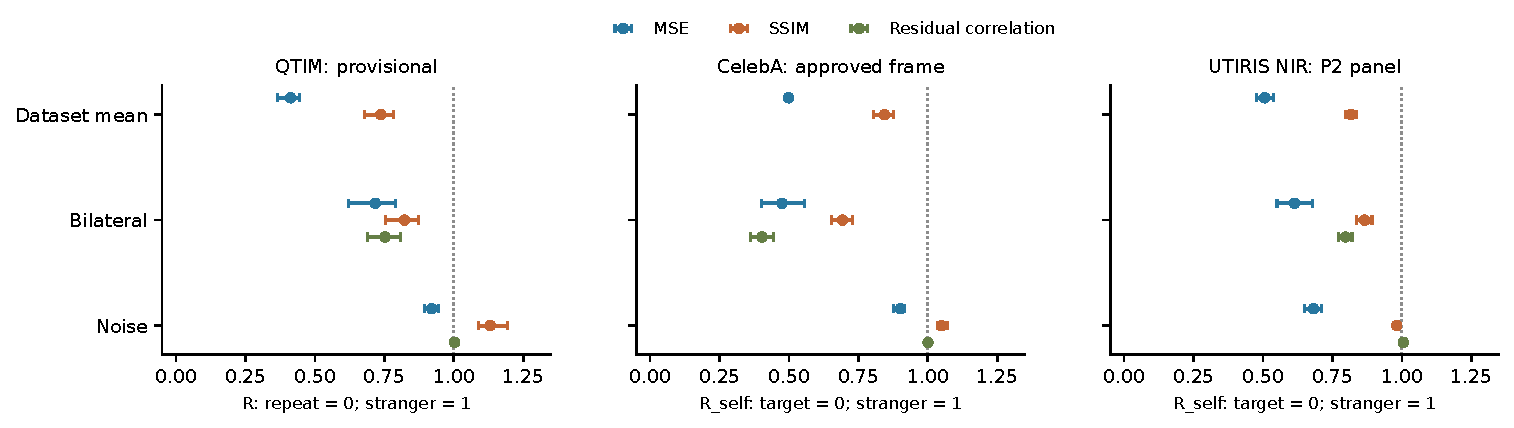
\includegraphics[width=\textwidth]{fig/audit_profiles.pdf}
\caption{Mean, bilateral and noise controls show different metric profiles.
QTIM uses the repeat anchor and remains provisional; CelebA and UTIRIS use self anchors.
The absent residual-correlation point at the mean is undefined.
Sources: the saved brain, face and iris metric-panel JSONs; generated by the paper preparation script.}
\end{figure}

\section{Reproducibility and outstanding author inputs}
The manuscript preparation is independent of historical absolute data paths and operates from the repository root.
The human-image experiment pipelines retain source-specific model and data requirements, and their presence in Git does not establish execution on this host.
The base face pipeline, latest fundus metric run, and full iris P3 require safe exports from their owners.
The atlas supplied here replaces the stale brain row with saved Gaussian aggregate panels and records every assembly transformation.
It does not recompute the maps from the private data, and its scalar annotations summarize pooled source errors rather than only the displayed axial slice.

The related ISBI source is preserved.
Publication overlap, dataset-specific ethics statements, portal requirements, and final author approval remain separate from successful typesetting.
No push is performed before the author reviews the rendered PDFs.
